\chapter{ピクセル解析ツールと読み出し試験デモンストレーション}
品質試験項目の1つである読み出し試験のデモンストレーションを学内実験室にて行った。
デモンストレーションの内容としては、4章で述べた2月にCERNで行ったチュートリアルとほぼ同じ内容である。
この章の前半では開発したツールと試験で使用するソフトウェアの概要について説明し、後にデモンストレーションの内容、各ソフトウェアの機能確認について述べる。

\section{ピクセル解析ツールの開発}
品質試験における読み出し試験では、3章で述べたようにモジュールの性能確認のためにピクセル解析を行う。
これを円滑に行うために、ピクセル解析ツールを開発した。また開発した解析ツールをローカルデータベースシステムに組み込んだ。
このツールについての詳細を以下に示す。

\subsection{概要}
YARRで読み出し試験を行った場合、結果ファイルはdigital scanやthreshold scanと言ったように各項目ごとにわかれて生成される。
また各結果ファイルにはモジュール上の全ピクセル結果がJSONの形で保存されている。
結果ファイルを模式的に表したものを以下に示す。

一方、品質試験の不良ピクセル解析においては、いくつかの試験結果を統一的に扱い、かつ各ピクセルごとに解析を行う必要がある。
そこで、開発した解析ツールでは複数の結果ファイルを1つのファイルにまとめ、ピクセルごとの解析処理を単純化する役割を担っている。
開発にはPythonとC++を用いた。またCERNが提供している解析フレームワークであるROOTを使用し、いくつかの試験データの統一ファイルとして、ROOT内部の機能であるTreeを使用した。
イメージを図\ref{analysis_tool_motivation}に示す。

\begin{figure}[bpt]\centering
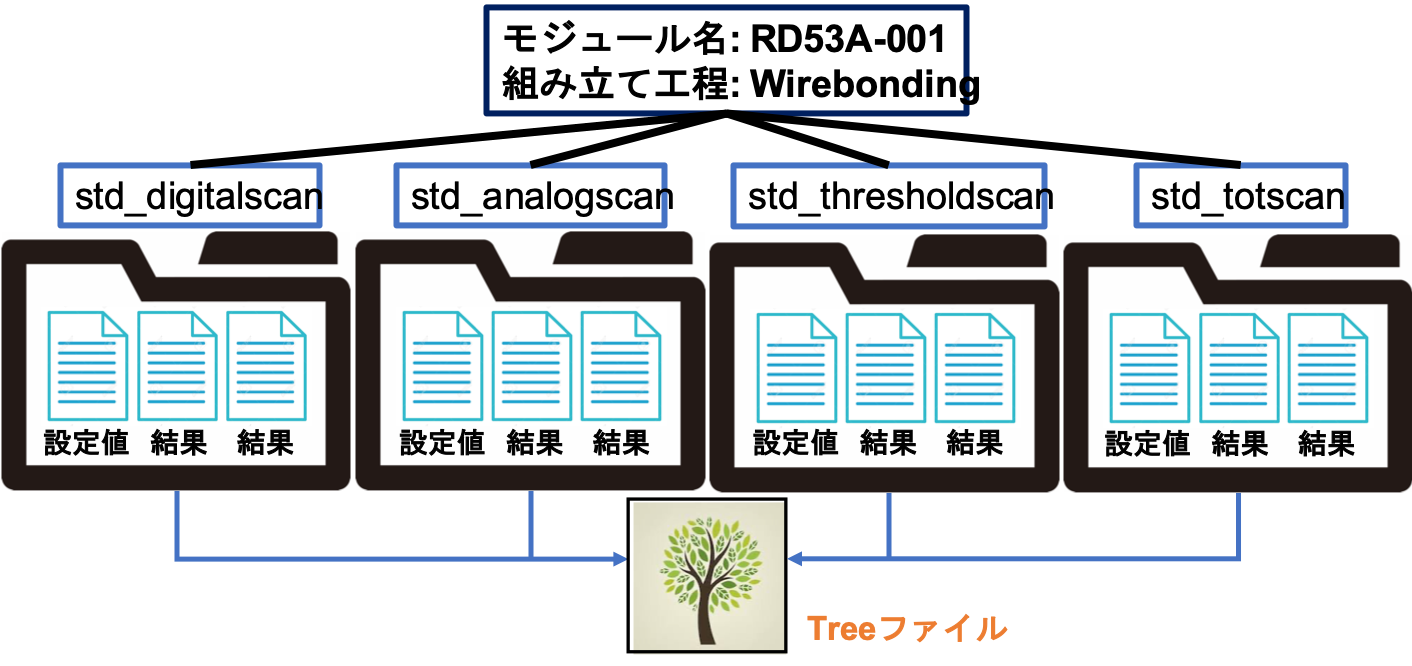
\includegraphics[width=12cm]{analysis_tool_motivation}
\caption[ピクセル解析ツール開発の動機]{ピクセル解析ツール開発の動機}
\label{analysis_tool_motivation}
\end{figure}

実際に作ったTreeファイルと、このファイルのデータ保持のイメージを図\ref{analysis_tool_tree}に示す。

\begin{figure}[bpt]
  \begin{center}
  \begin{minipage}{0.4\hsize}
    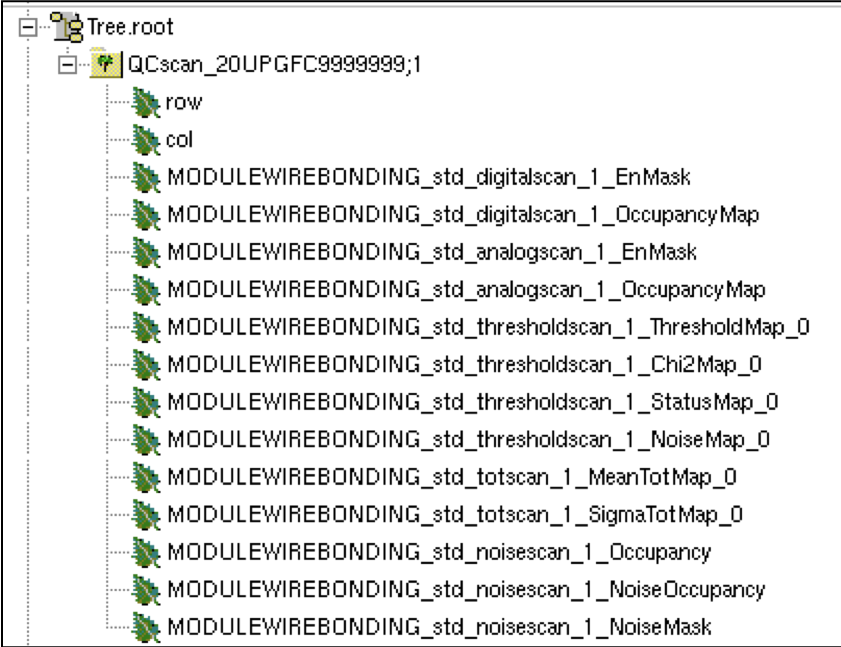
\includegraphics[width=8cm]{analysis_tool_tree_file}
  \end{minipage}
  \begin{minipage}{0.5\hsize}
    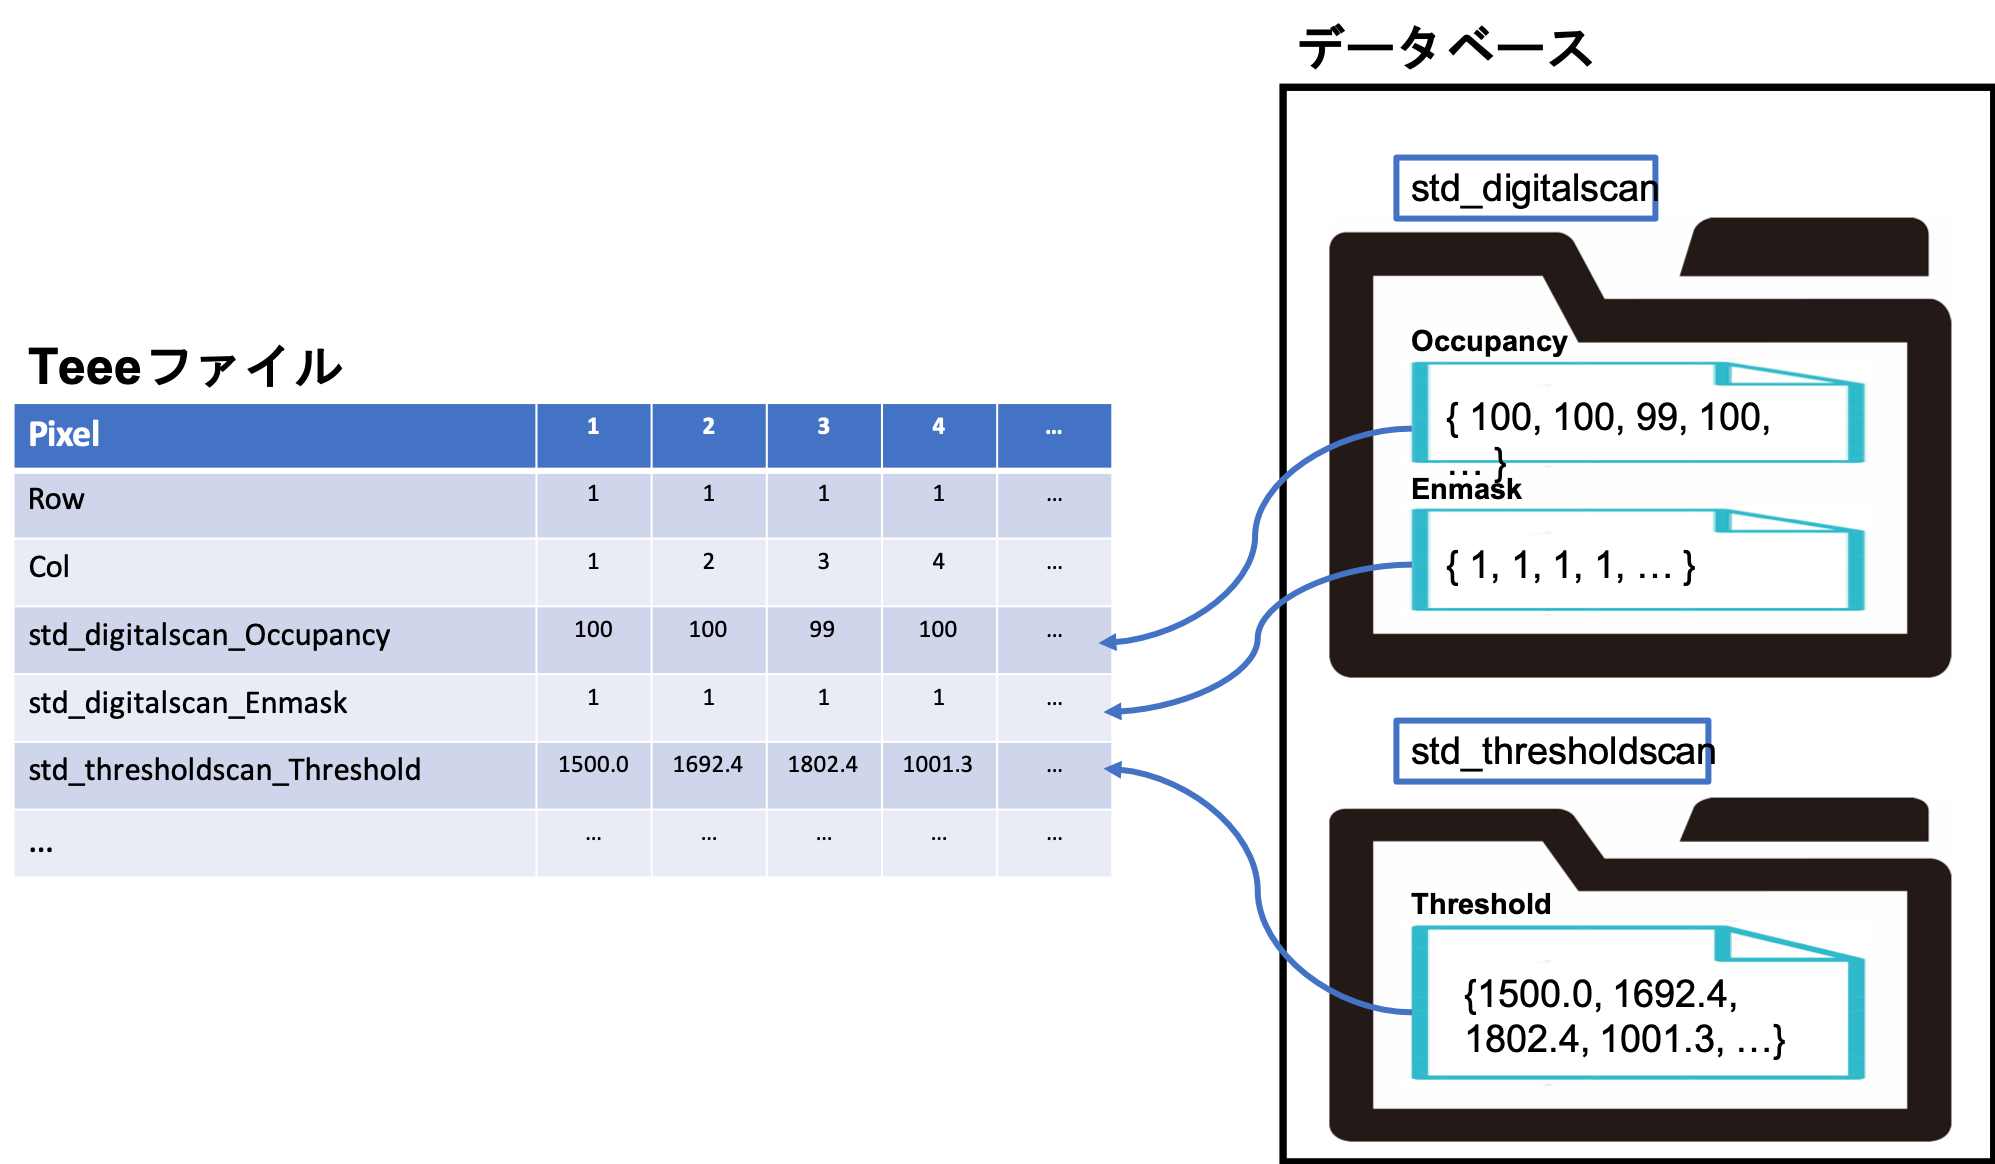
\includegraphics[width=8cm]{analysis_tool_tree_image}
  \end{minipage}
  \caption[Treeファイルとそのデータ保持]{Treeファイルとそのデータ保持}
  \label{analysis_tool_tree}
  \end{center}
\end{figure}

\subsection{ツールの内部構造と処理の流れ}
開発したツールは、主に以下で説明する3つの実行ファイルで構成される。それぞれの役割について説明する。

\begin{description}
  \item[getDataFile.py (Python)]\mbox{}\\ 
    データベースから対象となるデータファイルを取得、キャッシュファイルとしてサーバー上の一時ディレクトリに保存.
  \item[makeTree (C++)]\mbox{}\\ 
    getDataFile.pyを用いて生成されたキャッシュファイルを読み込み、Treeファイルを作成.
  \item[analysis (C++)]\mbox{}\\ 
  作成したTreeファイルを読み込み不良ピクセル解析を実行、結果値やプロットを出力.
\end{description}

処理の流れのイメージを図\ref{analysis_tool_flow}に示す。
処理を分けた理由について。
Python -> mongoとうまく共有する。
ROOTをC++主にsupport
makeTreeはformat、将来的に違う解析にも対応させたい。

\begin{figure}[bpt]\centering
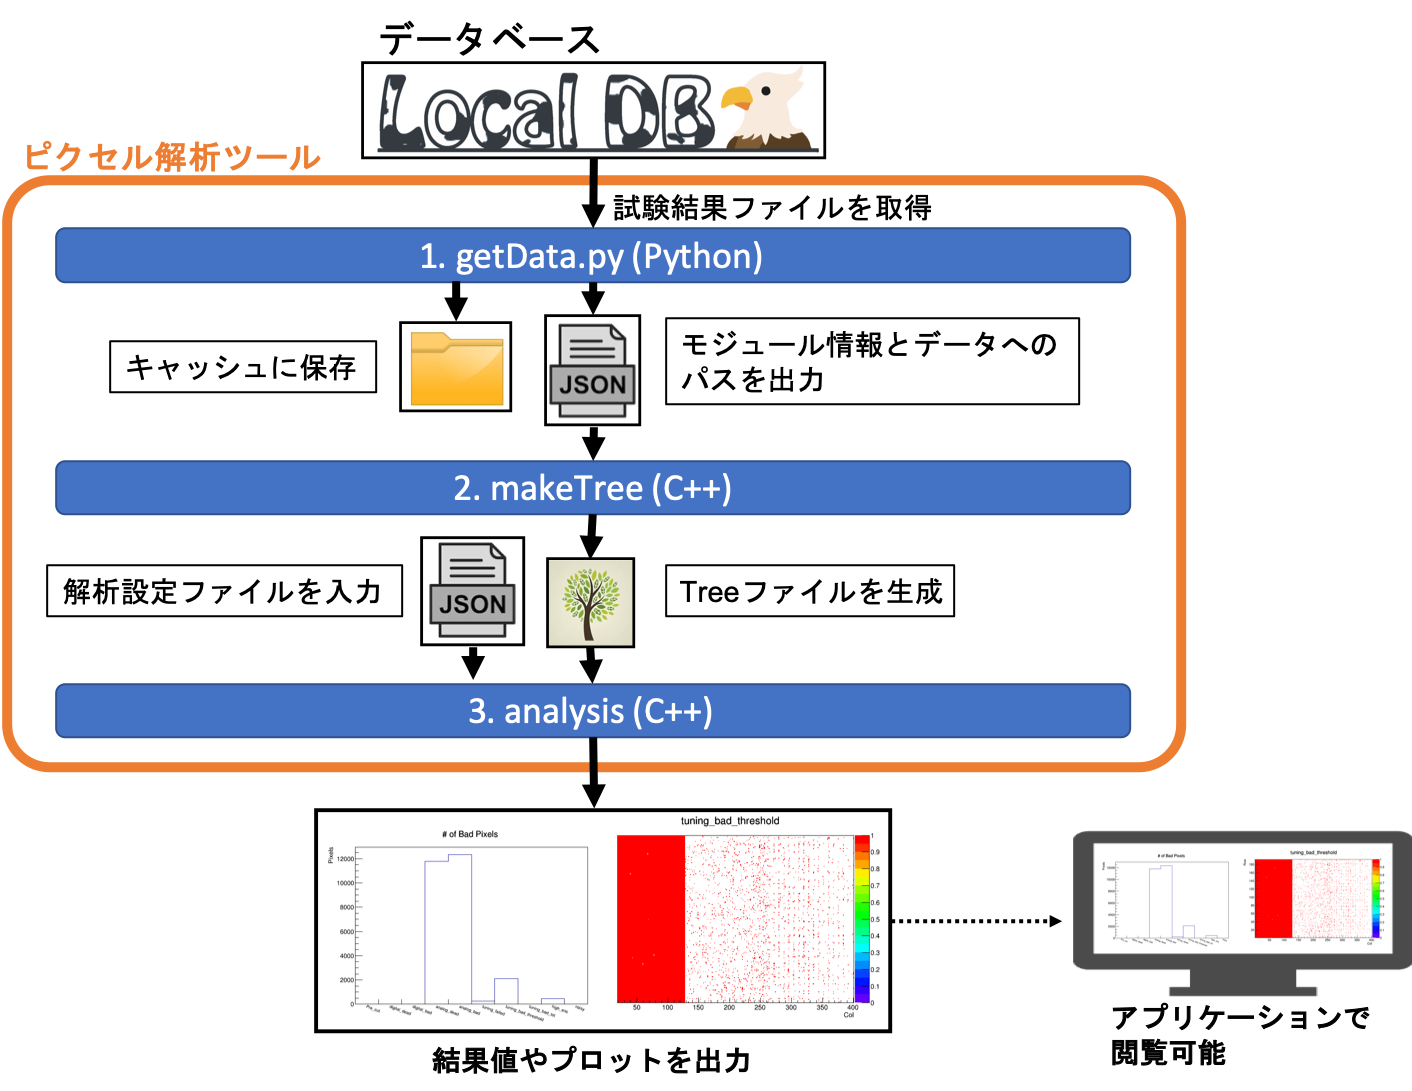
\includegraphics[width=12cm]{analysis_tool_flow}
\caption[ピクセル解析ツールの処理の流れ]{ピクセル解析ツールの処理の流れ}
\label{analysis_tool_flow}
\end{figure}

\newpage
\section{学内実験室におけるデモンストレーション}

上述したピクセル解析ツールを含む読み出し試験用ソフトウェアの機能確認を目的として、生産時における流れのデモンストレーションを学内実験室で行なった。
その詳細について以下に示す。

\subsection{用いたソフトウェアの概要}

試験で用いたソフトウェアをいかに示す。
また、これらソフトウェアの概要を図\ref{readout_SW_overview}に示す。
\begin{itemize}
  \item YARR
  \item MongoDB
  \item ウェブアプリケーション
  \item 中央データベースとのデータ同期ツール
  \item ピクセル解析ツール
  \item 時系列データ用データベース(InfluxDB)
    \begin{itemize}
      \item 時系列情報に特化したデータベース。このシステムにおいては温度、電圧などDCS情報を時間と共に保存、閲覧するために用いる。
    \end{itemize}
  \item InfluxDB解析ソフト(Grafana)
    \begin{itemize}
      \item InfluxDBに保存された情報の解析、閲覧に用いる。ウェブブラウザー上でデータを閲覧することができる。
    \end{itemize}
  \item 電源操作用ソフト
    \begin{itemize}
      \item 電源を遠隔で操作し、モジュールに電圧を供給する。また電圧、電流値を取得し、InfluxDBにアップロードする。
    \end{itemize}
  \item 温度読み出し用ソフト
    \begin{itemize}
      \item モジュールに付属しているサーミスタの温度を取得し、InfluxDBにアップロードする。
    \end{itemize}
\end{itemize}

\begin{figure}[bpt]\centering

\includegraphics[width=8cm]{figure}
\caption[読み出し試験に用いるソフトウェアの概要]{読み出し試験に用いるソフトウェアの概要}
\label{readout_SW_overview}
\end{figure}

\subsection{用いたハードウェア}
読み出し試験に用いたハードウェアについて、以下に詳細を記す。

\subsubsection{RD53Aシングルモジュール(RD53A Single Chip Card, SCC)}
今回読み出しに使うモジュールとして、研究室で所有しているRD53Aシングルモジュール(RD53A Single Chip Card, SCC)を使用した。
SCCは試験用に作られたFEチップを一枚搭載するモジュールである。今回の実験ではシリコンセンサーを持たないものを使用した。
SCCはFEチップ電源端子、データ転送端子をもち、読み出しを行う際はそれぞれ配線をする。
FEチップ付近にはNTCサーミスタを搭載していて、ボード上の端子からその抵抗値を取得することで温度を測定することができる。
図\ref{demo_rd53a_SCC}に写真を示す。

\begin{figure}[h]\centering
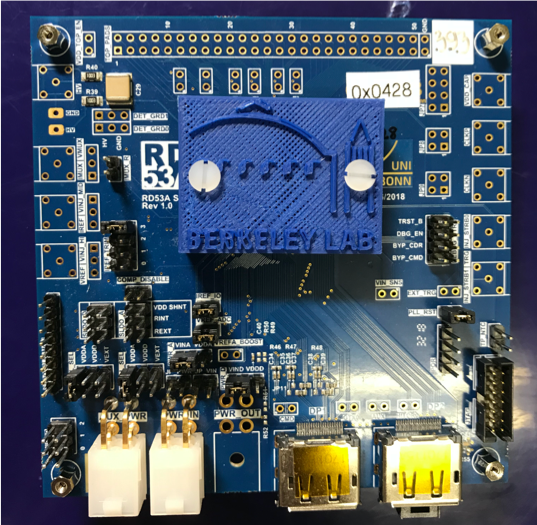
\includegraphics[width=8cm]{rd53a_SCC}
\caption[RD53A]{RD53A}
\label{demo_rd53a_SCC}
\end{figure}

\subsubsection{電源}
モジュールの電圧供給にKEYSIGHTのE3646A 60Wデュアル出力電源\cite{1}(図\ref{demo_power_supply})を用いた。
\begin{figure}[h]\centering
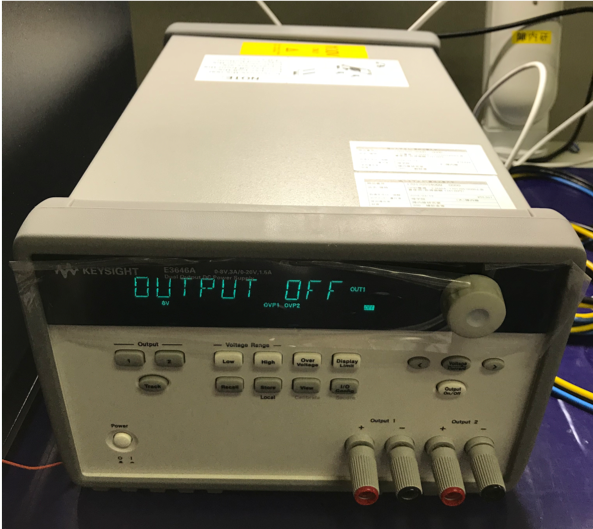
\includegraphics[width=8cm]{power_supply}
\caption[電源]{電源}
\label{demo_power_supply}
\end{figure}

\subsubsection{モジュールサーミスタ温度読み出しシステム}
モジュールに付属しているサーミスタを用いて温度の読み出し装置を作成した。
このシステムの中で扱った装置を表\ref{demo_temp_device}にまとめた。
サーミスタの抵抗値変化をADCとRaspberry Piを用いて読み出す回路を作成した。
回路図、実際に配線した様子を図\ref{demo_temp_circit_pic}に示す。

\begin{table}[tbp]
\begin{center}
\caption[hoge]{hoge}
\label{demo_temp_device}
  \begin{tabular}{|ll|} \hline
    装置 & 機種 \\ \hline
    10$\rm{k\Omega}$抵抗 & - \\
    ADC & MCP3002\cite{3} \\  
    RaspberryPi &  Raspberry Pi 3 Model B Plus Rev 1.3\cite{4} \\ \hline 
  \end{tabular}
\end{center}
\end{table}

\begin{figure}[h]\centering
  \begin{minipage}{0.5\hsize}
    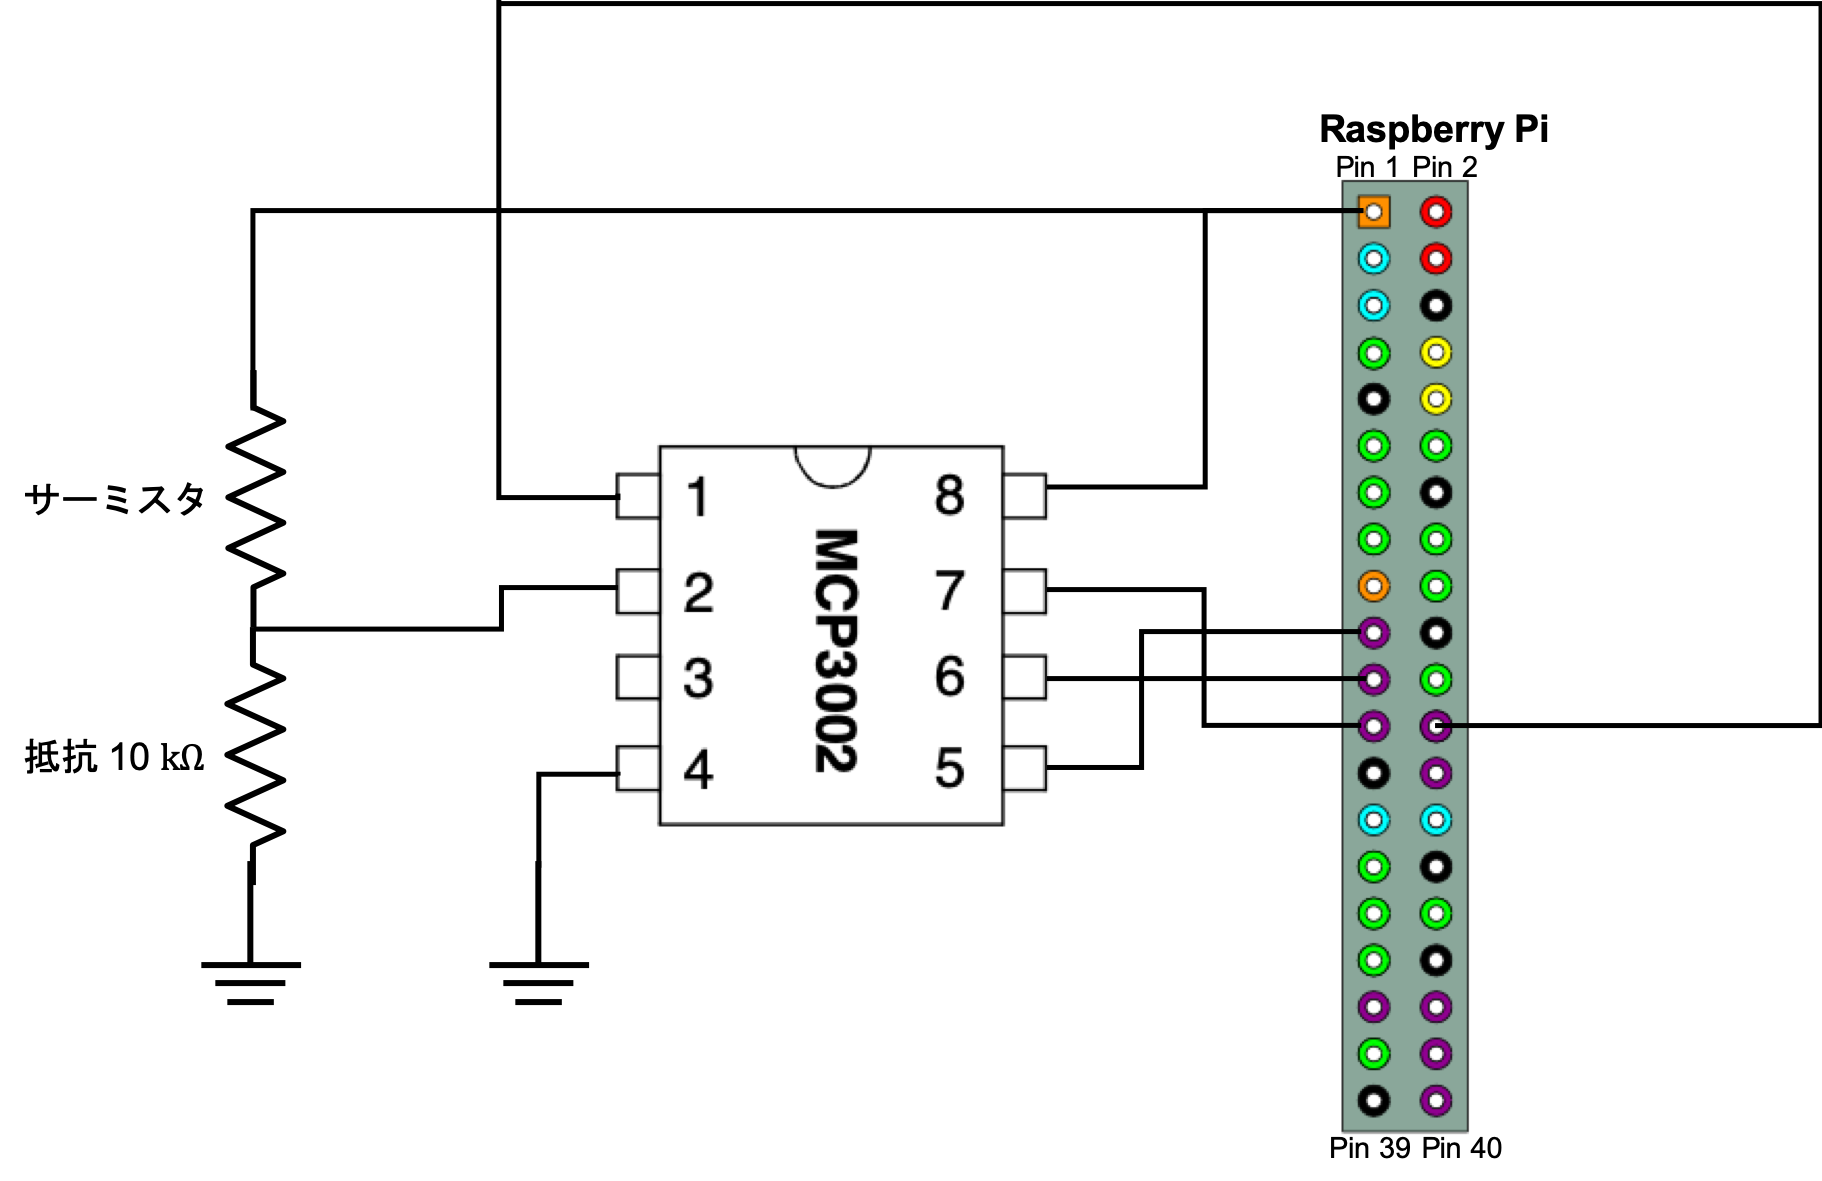
\includegraphics[width=8cm]{temp_circit}
  \end{minipage}
  \begin{minipage}{0.5\hsize}
    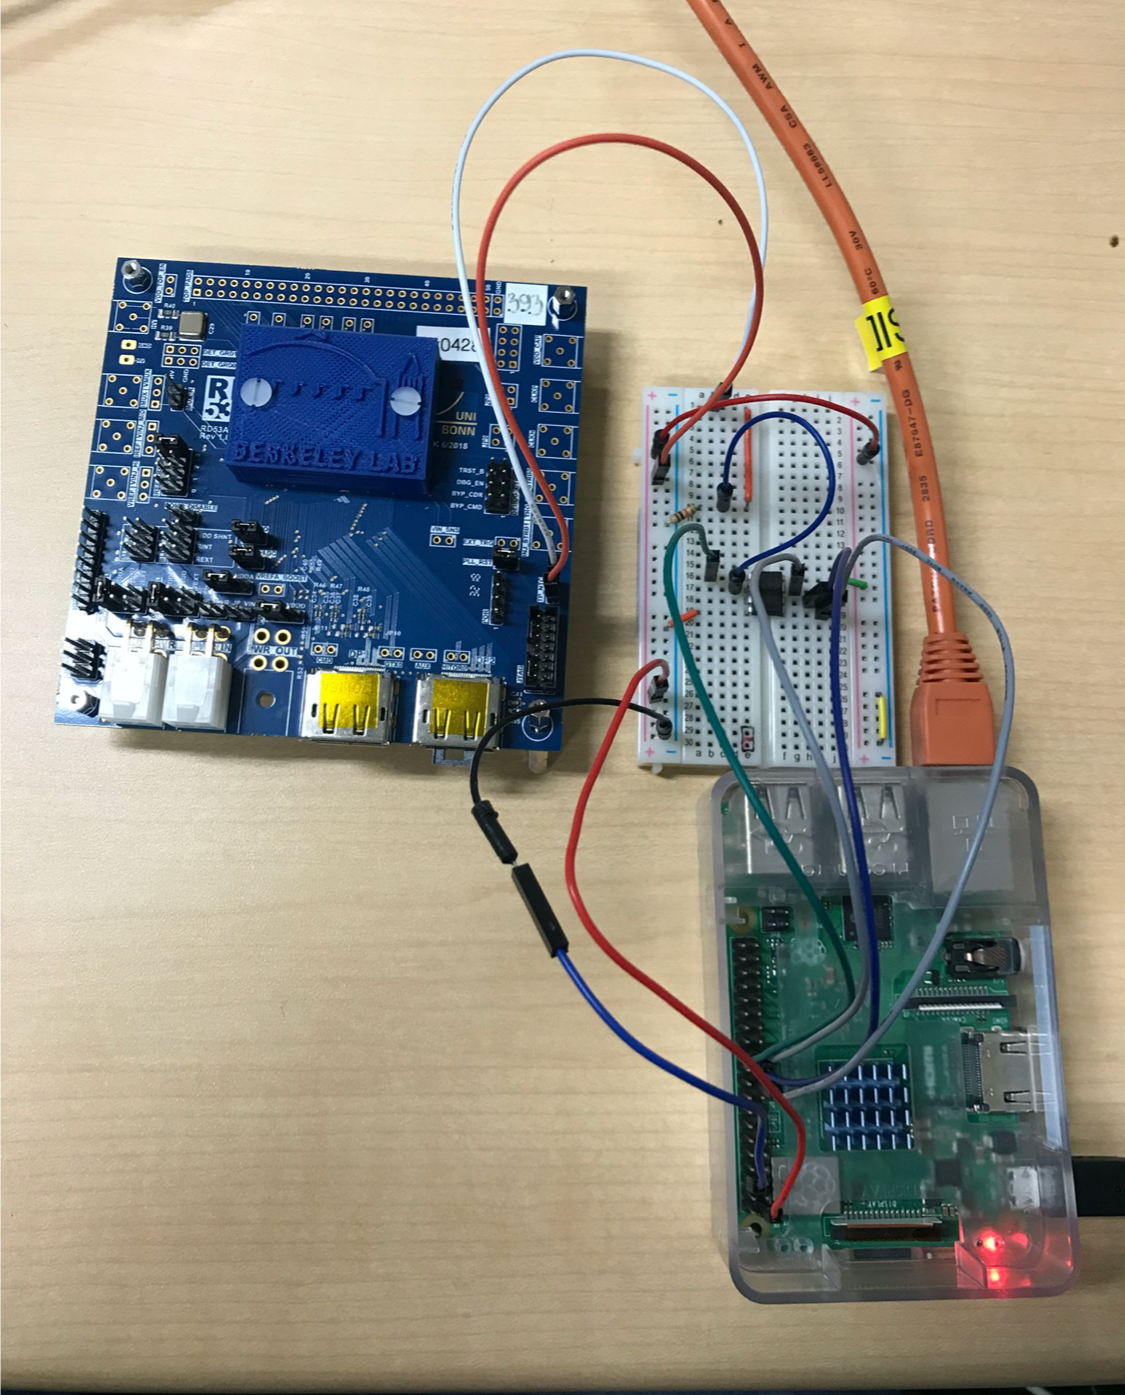
\includegraphics[width=6cm]{temp_circit_pic}
  \end{minipage}
\caption[モジュール付属サーミスタを用いた温度読み出し回路]{モジュール付属サーミスタを用いた温度読み出し回路}
\label{demo_temp_circit_pic}
\end{figure}

\subsubsection{FPGAボード}

FPGAボードにXpressK7\cite{2}(図\ref{demo_fpga_board})を用いた。
\begin{figure}[h]\centering
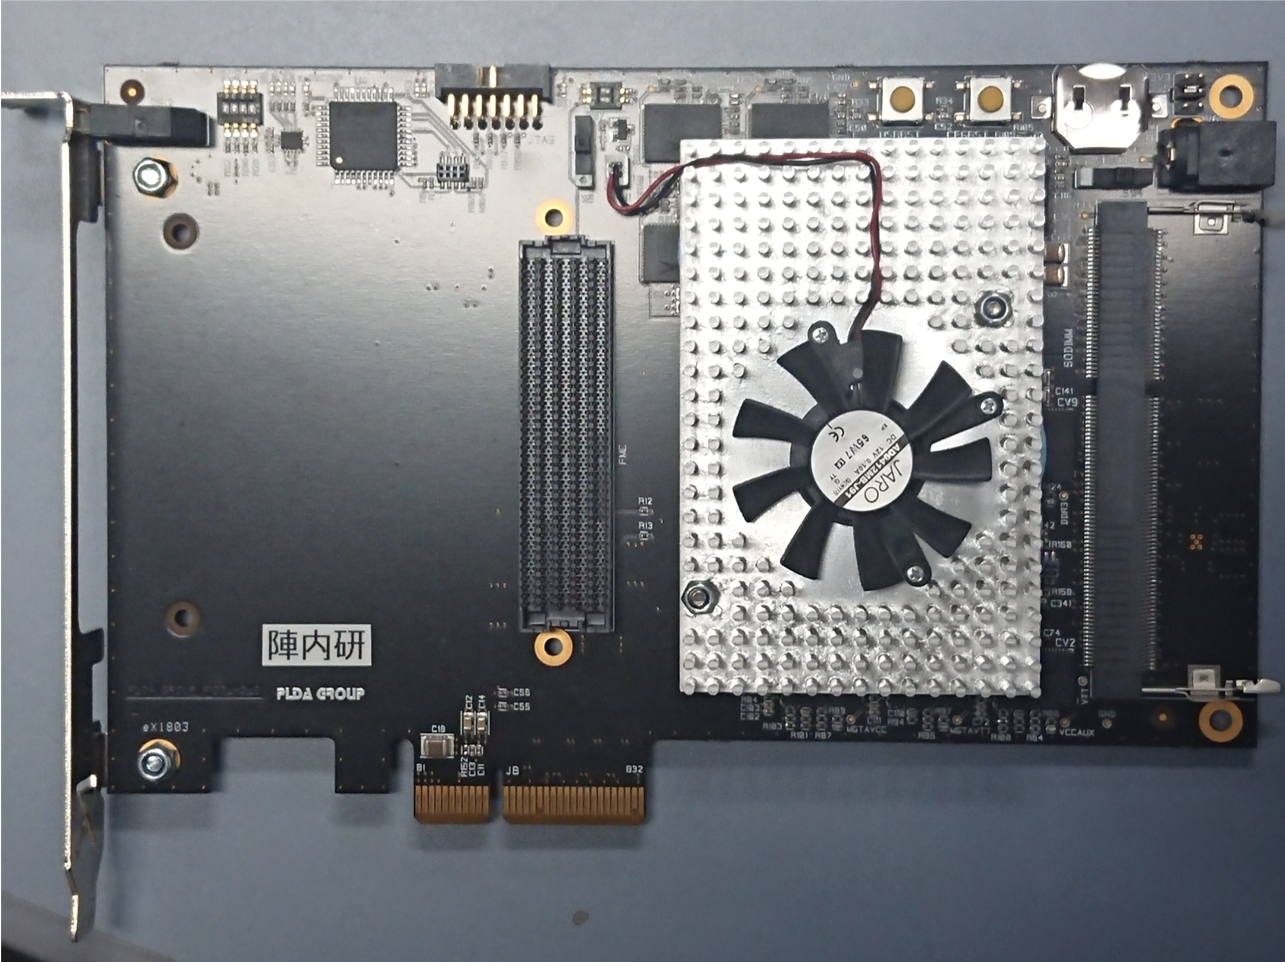
\includegraphics[width=8cm]{fpga_board}
\caption[FPGAボード]{FPGAボード}
\label{demo_fpga_board}
\end{figure}

\subsubsection{FMC-DisplayPort変換カード}

今回使用したFMC-DisplayPort変換カード(Ohio Card)を図\ref{demo_ohio}に示す。
\begin{figure}[h]\centering

\includegraphics[width=8cm]{figure}
\caption[オハイオ]{オハイオ}
\label{demo_ohio}
\end{figure}

\subsubsection{PC}
今回用いたPCの性能を以下に示す。

\subsubsection{セットアップ}
読み出し試験に用いるハードウェアのセットアップを概要を図\ref{readout_setup_overview}に示す。

\begin{figure}[bpt]\centering
  \begin{minipage}{0.5\hsize}
    %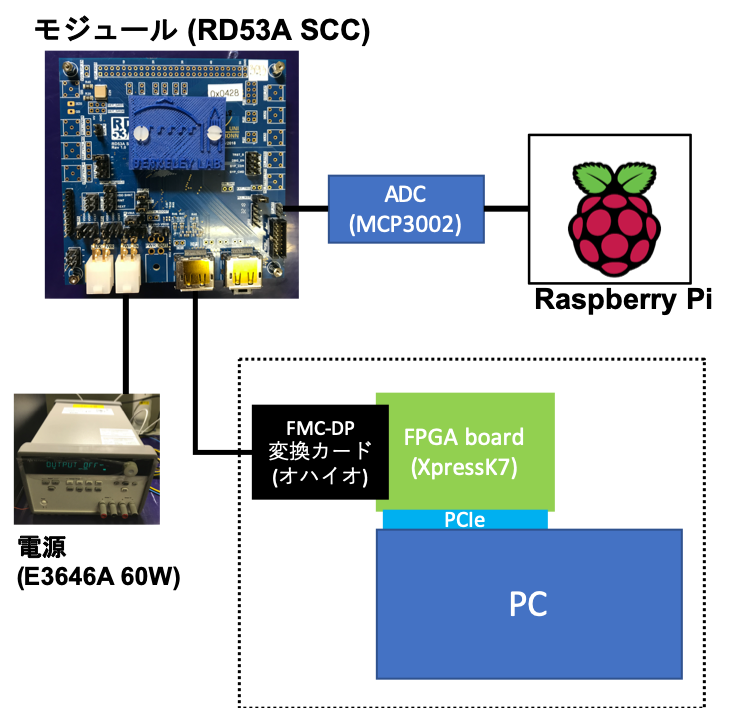
\includegraphics[width=8cm]{HW_setup}
    
\includegraphics[width=8cm]{figure}
  \end{minipage}
  \begin{minipage}{0.5\hsize}
    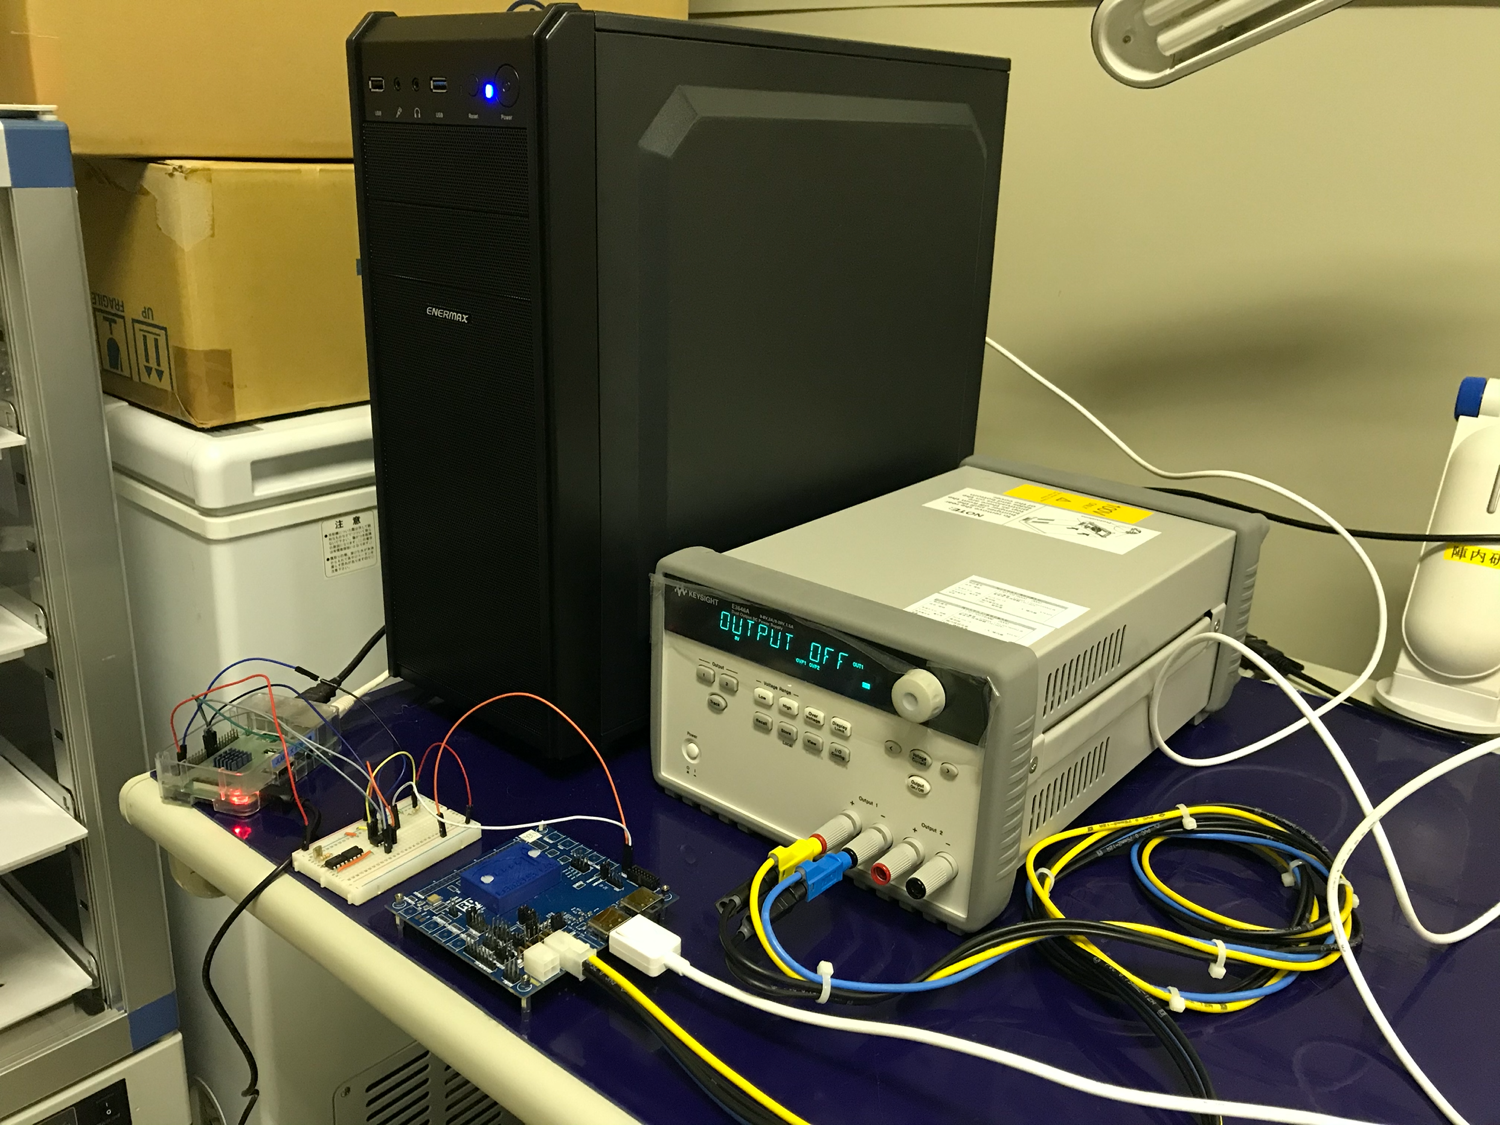
\includegraphics[width=7cm]{HW_setup_pic}
  \end{minipage}
\caption[ハードウェアセットアップの概要]{ハードウェアセットアップの概要}
\label{readout_setup_overview}
\end{figure}


\subsection{デモンストレーションの流れ}

今回のデモンストレーションで確認した機能を以下に示す。
\begin{itemize}
  \item 中央データベースとローカルデータベースの同期.(モジュール情報、読み出し試験結果)
  \item 読み出し試験に使う各種機能.
   \begin{itemize}
     \item 試験実施と結果のアップロード.
     \item DCS情報の取得、監視.
     \item 試験結果検索.
     \item 試験結果閲覧.
   \end{itemize}
  \item 結果選択とピクセル解析機能.
\end{itemize}

またデモンストレーションにおける流れの概要を図\ref{demo_flow}に示す。

\begin{figure}[bpt]\centering

\includegraphics[width=1cm]{figure}
\caption[デモンストレーションの流れ]{デモンストレーションの流れ}
\label{demo_flow}
\end{figure}


\subsection{機能確認}
読み出し試験を通して、各ソフトウェア機能が正しく動くことを確認した。
詳細を以下に記す。

\subsubsection{中央データベースからモジュール情報のダウンロード}
ダウンロードし、ウェブアプリケーションで確認した。
確認した画面を図\ref{demo_download_SCC}に示す。
今回行った試験結果はこのモジュールに紐つける形でローカルデータベースに保存される。

\begin{figure}[bpt]\centering
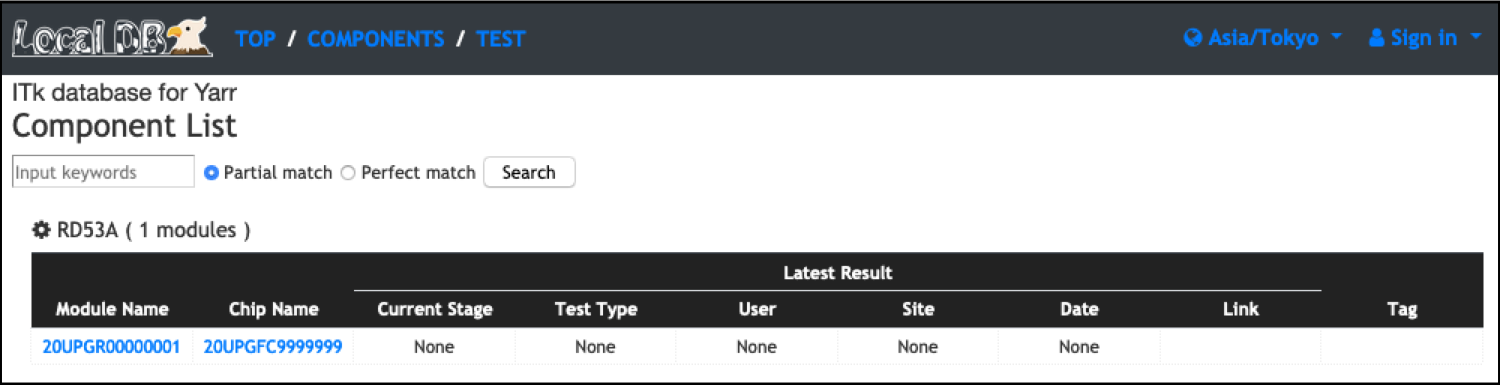
\includegraphics[width=1cm]{demo_download_SCC}
\caption[ダウンロードしたモジュールID確認画面]{ダウンロードしたモジュールID確認画面}
\label{demo_download_SCC}
\end{figure}

%%%%%%%%%%%%%%%%%%%%%%%%%%%%%%%%%%%%%%%%%%%%%%%%%
%%%%%%%%%%%%%%%%%%%%%%%%%%%%%%%%%%%%%%%%%%%%%%%%%

\subsubsection{読み出し試験実施}
以下の流れに沿って読み出しを行ない、結果をローカルデータベースにアップロードした。
\begin{enumerate}
  \item デジタル回路読み出し(\texttt{std$\_$digitalscan})
  \item アナログ回路読み出し(\texttt{std$\_$analogscan})
  \item 調整前Threshold測定(\texttt{std$\_$thresholdscan})
  \item Threshold調整
  \item ToT調整
  \item Threshold再調整
  \item 調整後Threshold測定
  \item ToT測定(\texttt{std$\_$totscan})
  \item ノイズ測定(\texttt{std$\_$noisescan})
\end{enumerate}
また読み出し試験を通してDCS情報は監視し、試験結果と同様にローカルデータベースにアップロードした。

%%%%%%%%%%%%%%%%%%%%%%%%%%%%%%%%%%%%%%%%%%%%%%%%%
%%%%%%%%%%%%%%%%%%%%%%%%%%%%%%%%%%%%%%%%%%%%%%%%%
\subsubsection{DCS情報の監視}
読み出し試験は、DCS情報を監視しながら行った。
それぞれの値は対応するソフトウェアを用いてInfluxDBにアップロードした。
その値をGrafanaを使って監視をした。その様子を図\ref{demo_monitor_dcs}に示す。

\begin{figure}[bpt]\centering
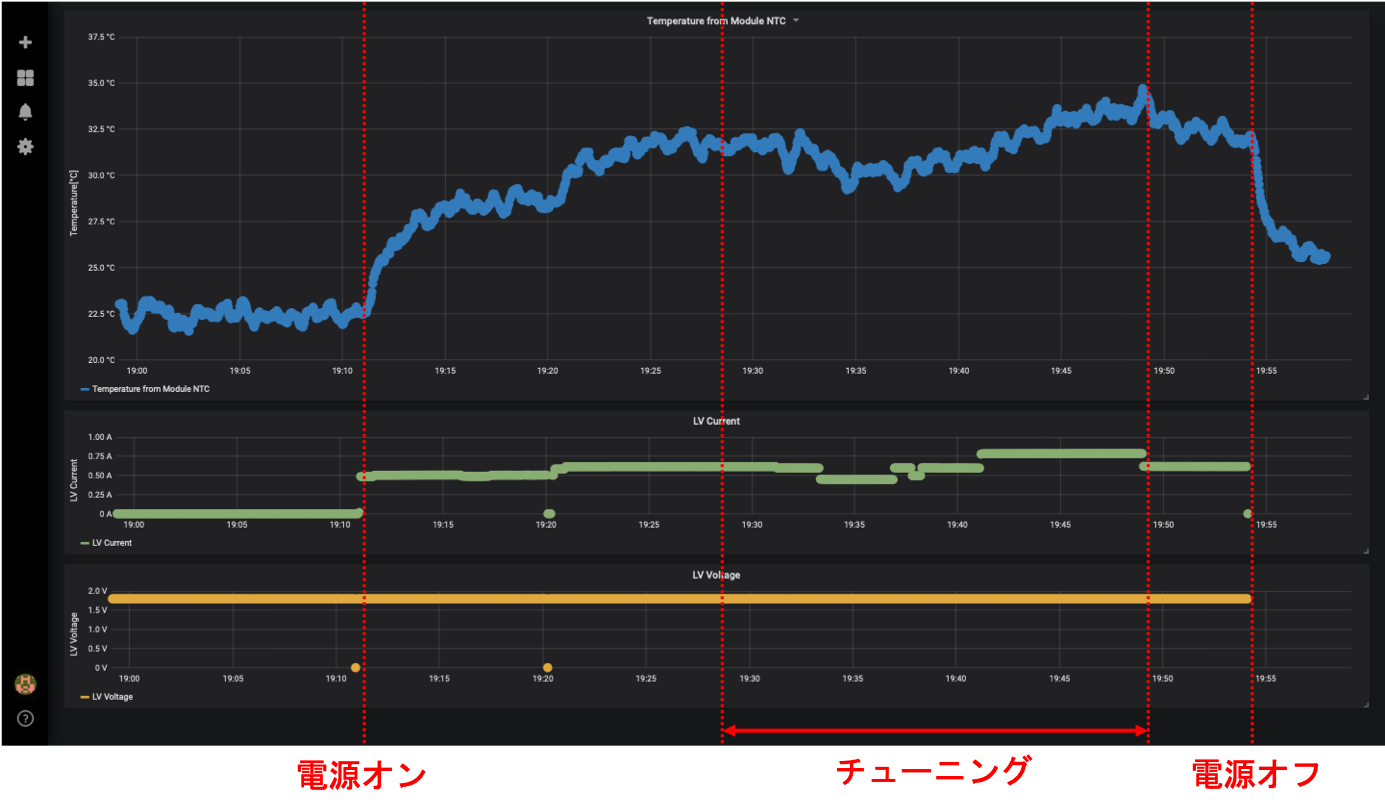
\includegraphics[width=12cm]{demo_monitor_dcs}
\caption[DCSのモニタリング]{DCSのモニタリング}
\label{demo_monitor_dcs}
\end{figure}

%%%%%%%%%%%%%%%%%%%%%%%%%%%%%%%%%%%%%%%%%%%%%%%%%
%%%%%%%%%%%%%%%%%%%%%%%%%%%%%%%%%%%%%%%%%%%%%%%%%
\newpage
\subsubsection{検索機能の確認}

検索機能の確認を行った。
\begin{figure}[bpt]\centering
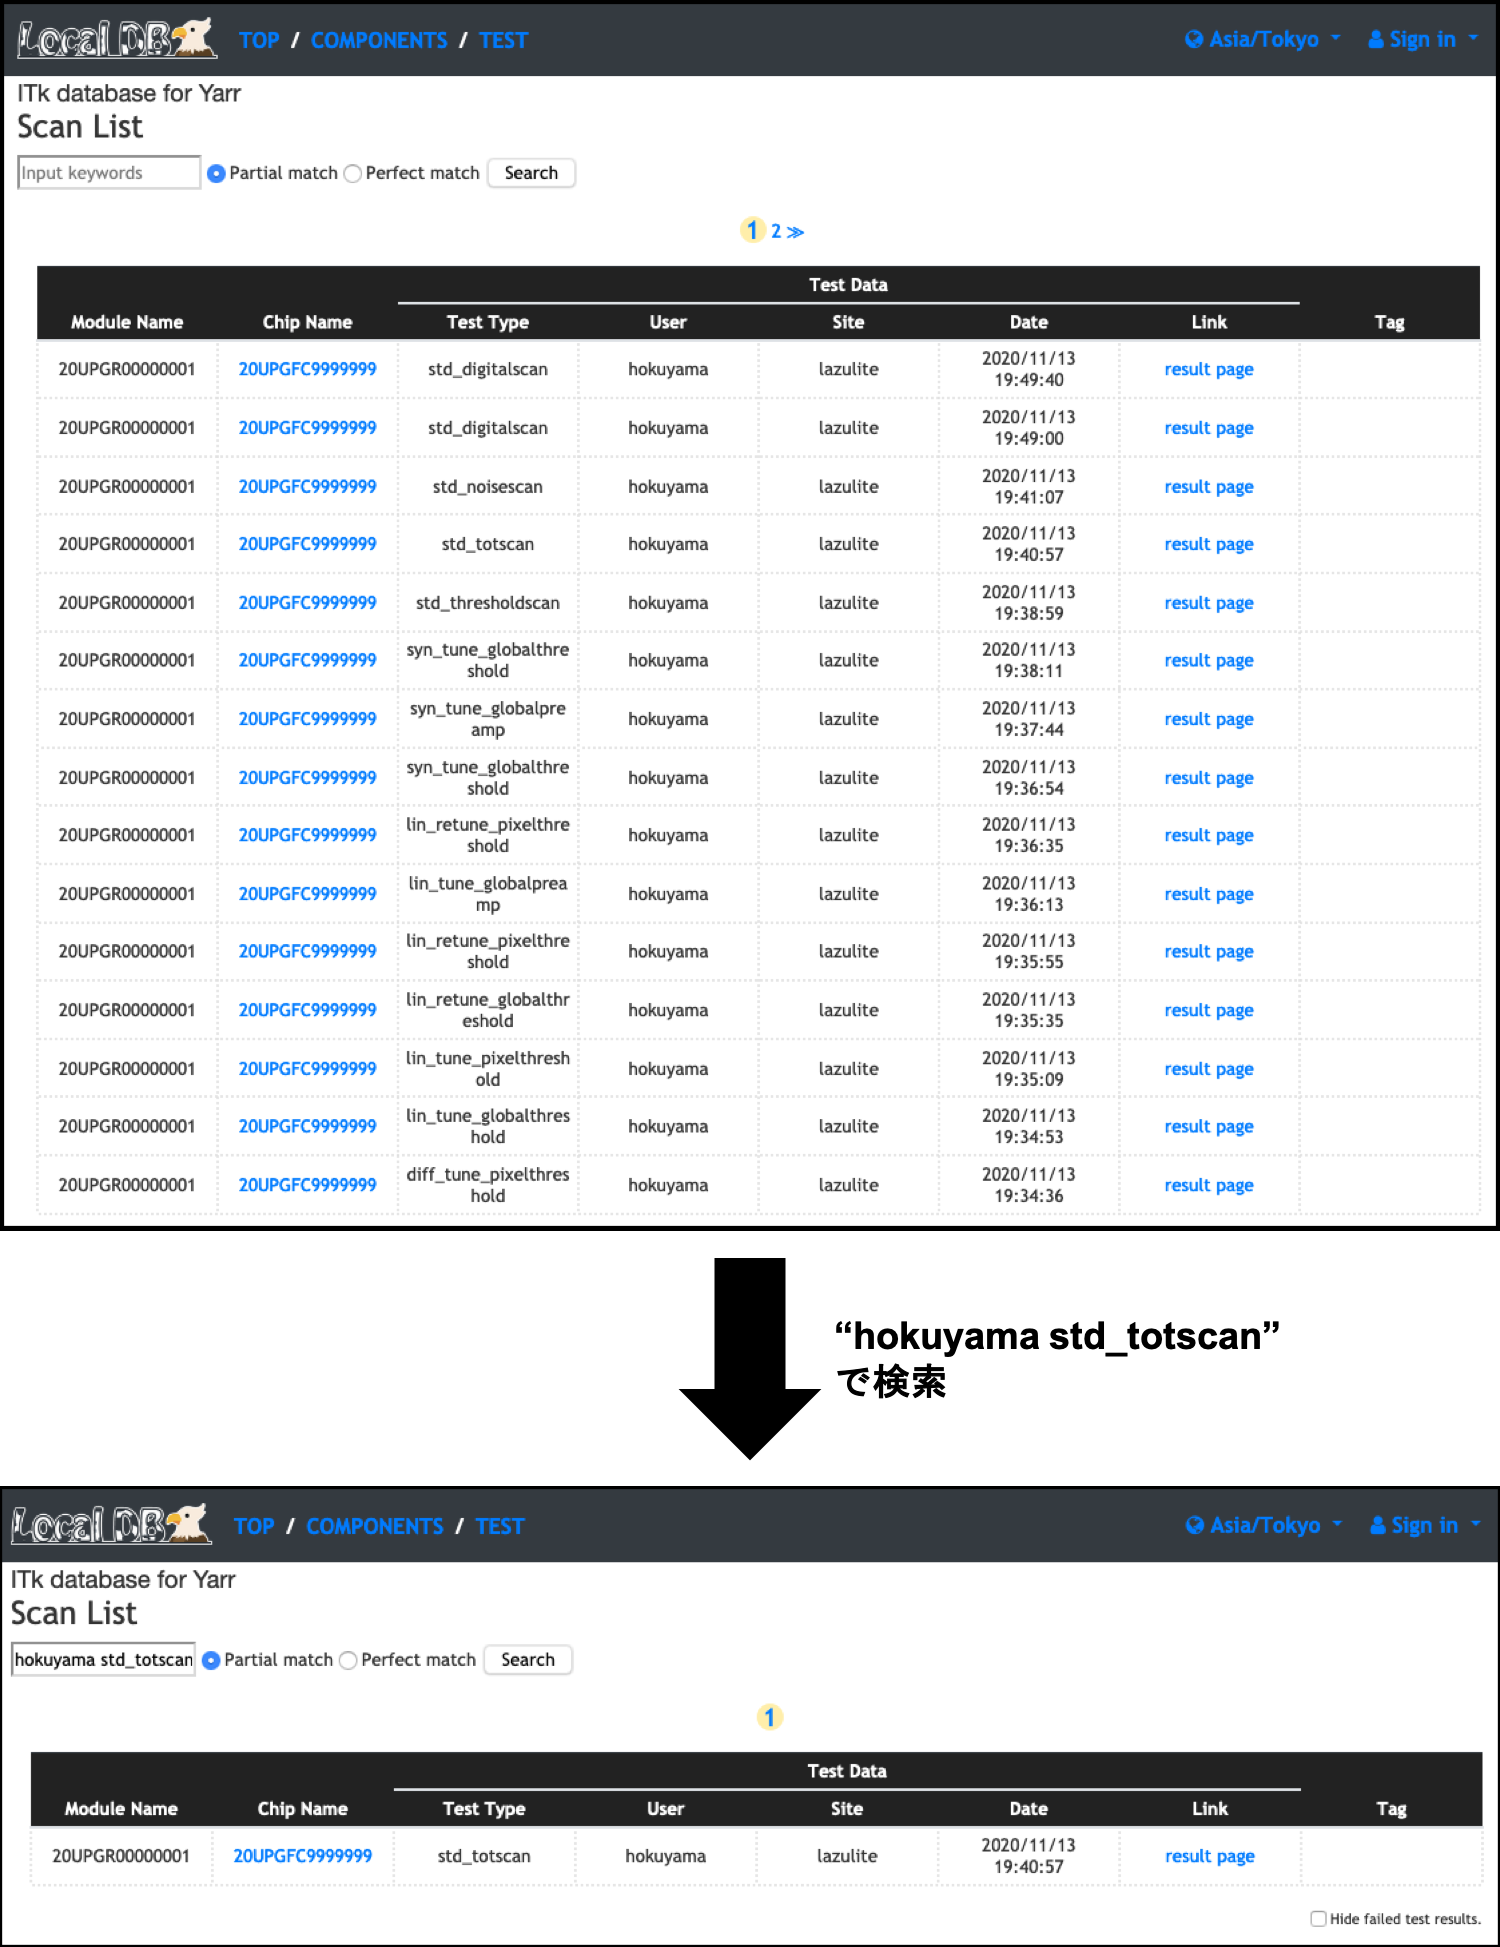
\includegraphics[width=12cm]{demo_search_function}
\caption[検索機能の確認]{検索機能の確認}
\label{demo_search_function}
\end{figure}

%%%%%%%%%%%%%%%%%%%%%%%%%%%%%%%%%%%%%%%%%%%%%%%%%
%%%%%%%%%%%%%%%%%%%%%%%%%%%%%%%%%%%%%%%%%%%%%%%%%
\newpage
\subsubsection{試験結果の閲覧}
ウェブアプリケーションを用いて、試験結果を閲覧した。その様子を図\ref{demo_view_result}に示す。
\begin{figure}[bpt]\centering
  \begin{center}
  \begin{minipage}{0.4\hsize}
    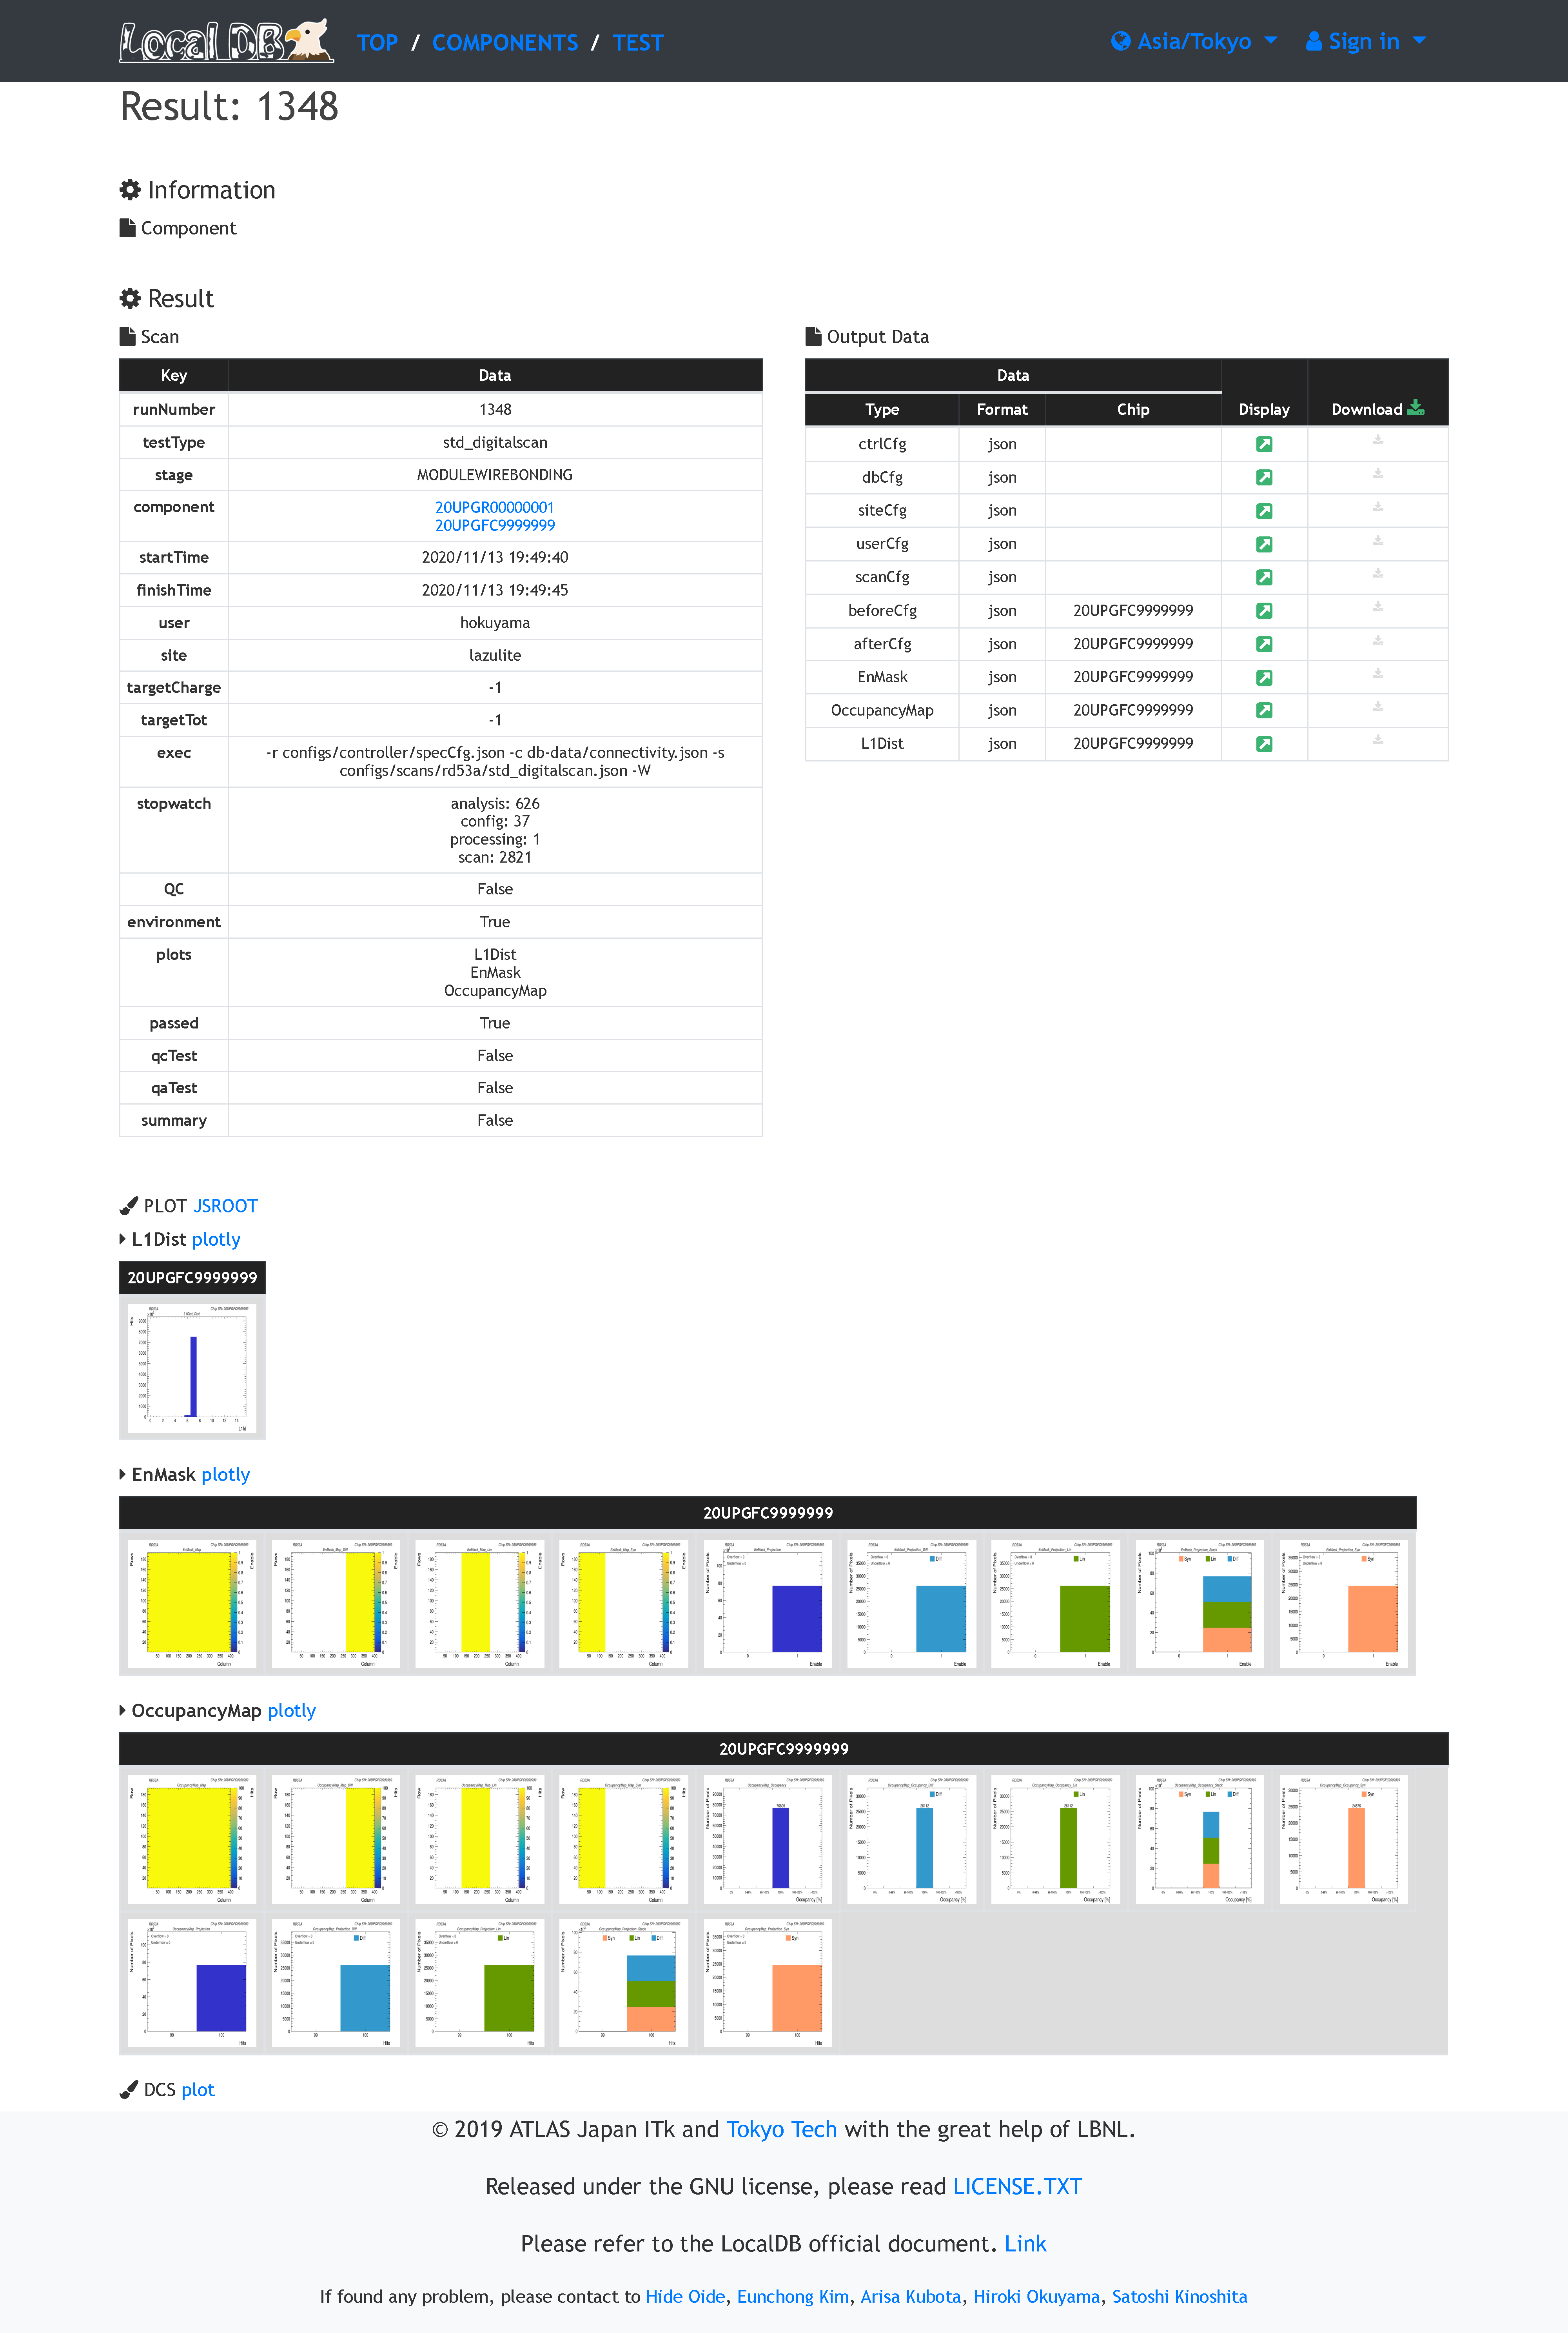
\includegraphics[width=65mm]{demo_view_scan_result}
  \end{minipage}
  \begin{minipage}{0.4\hsize}
    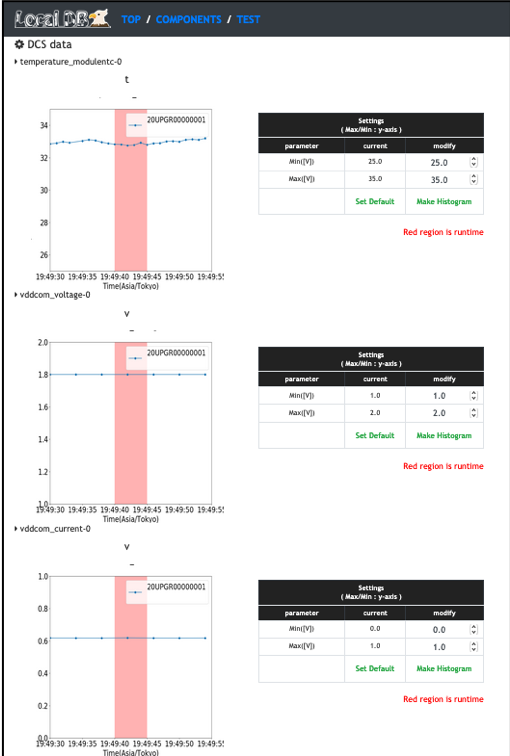
\includegraphics[width=7cm]{demo_view_dcs}
  \end{minipage}
  \caption[試験結果の閲覧]{試験結果の閲覧}
  \label{demo_view_result}
  \end{center}
\end{figure}


%%%%%%%%%%%%%%%%%%%%%%%%%%%%%%%%%%%%%%%%%%%%%%%%%
%%%%%%%%%%%%%%%%%%%%%%%%%%%%%%%%%%%%%%%%%%%%%%%%%
\newpage
\subsubsection{結果選択とピクセル解析}
読み出し結果を選択し、ピクセル解析を行なった。
結果選択の様子を図\ref{demo_select_scans}に示す。
\begin{figure}[bpt]\centering
  \begin{center}
    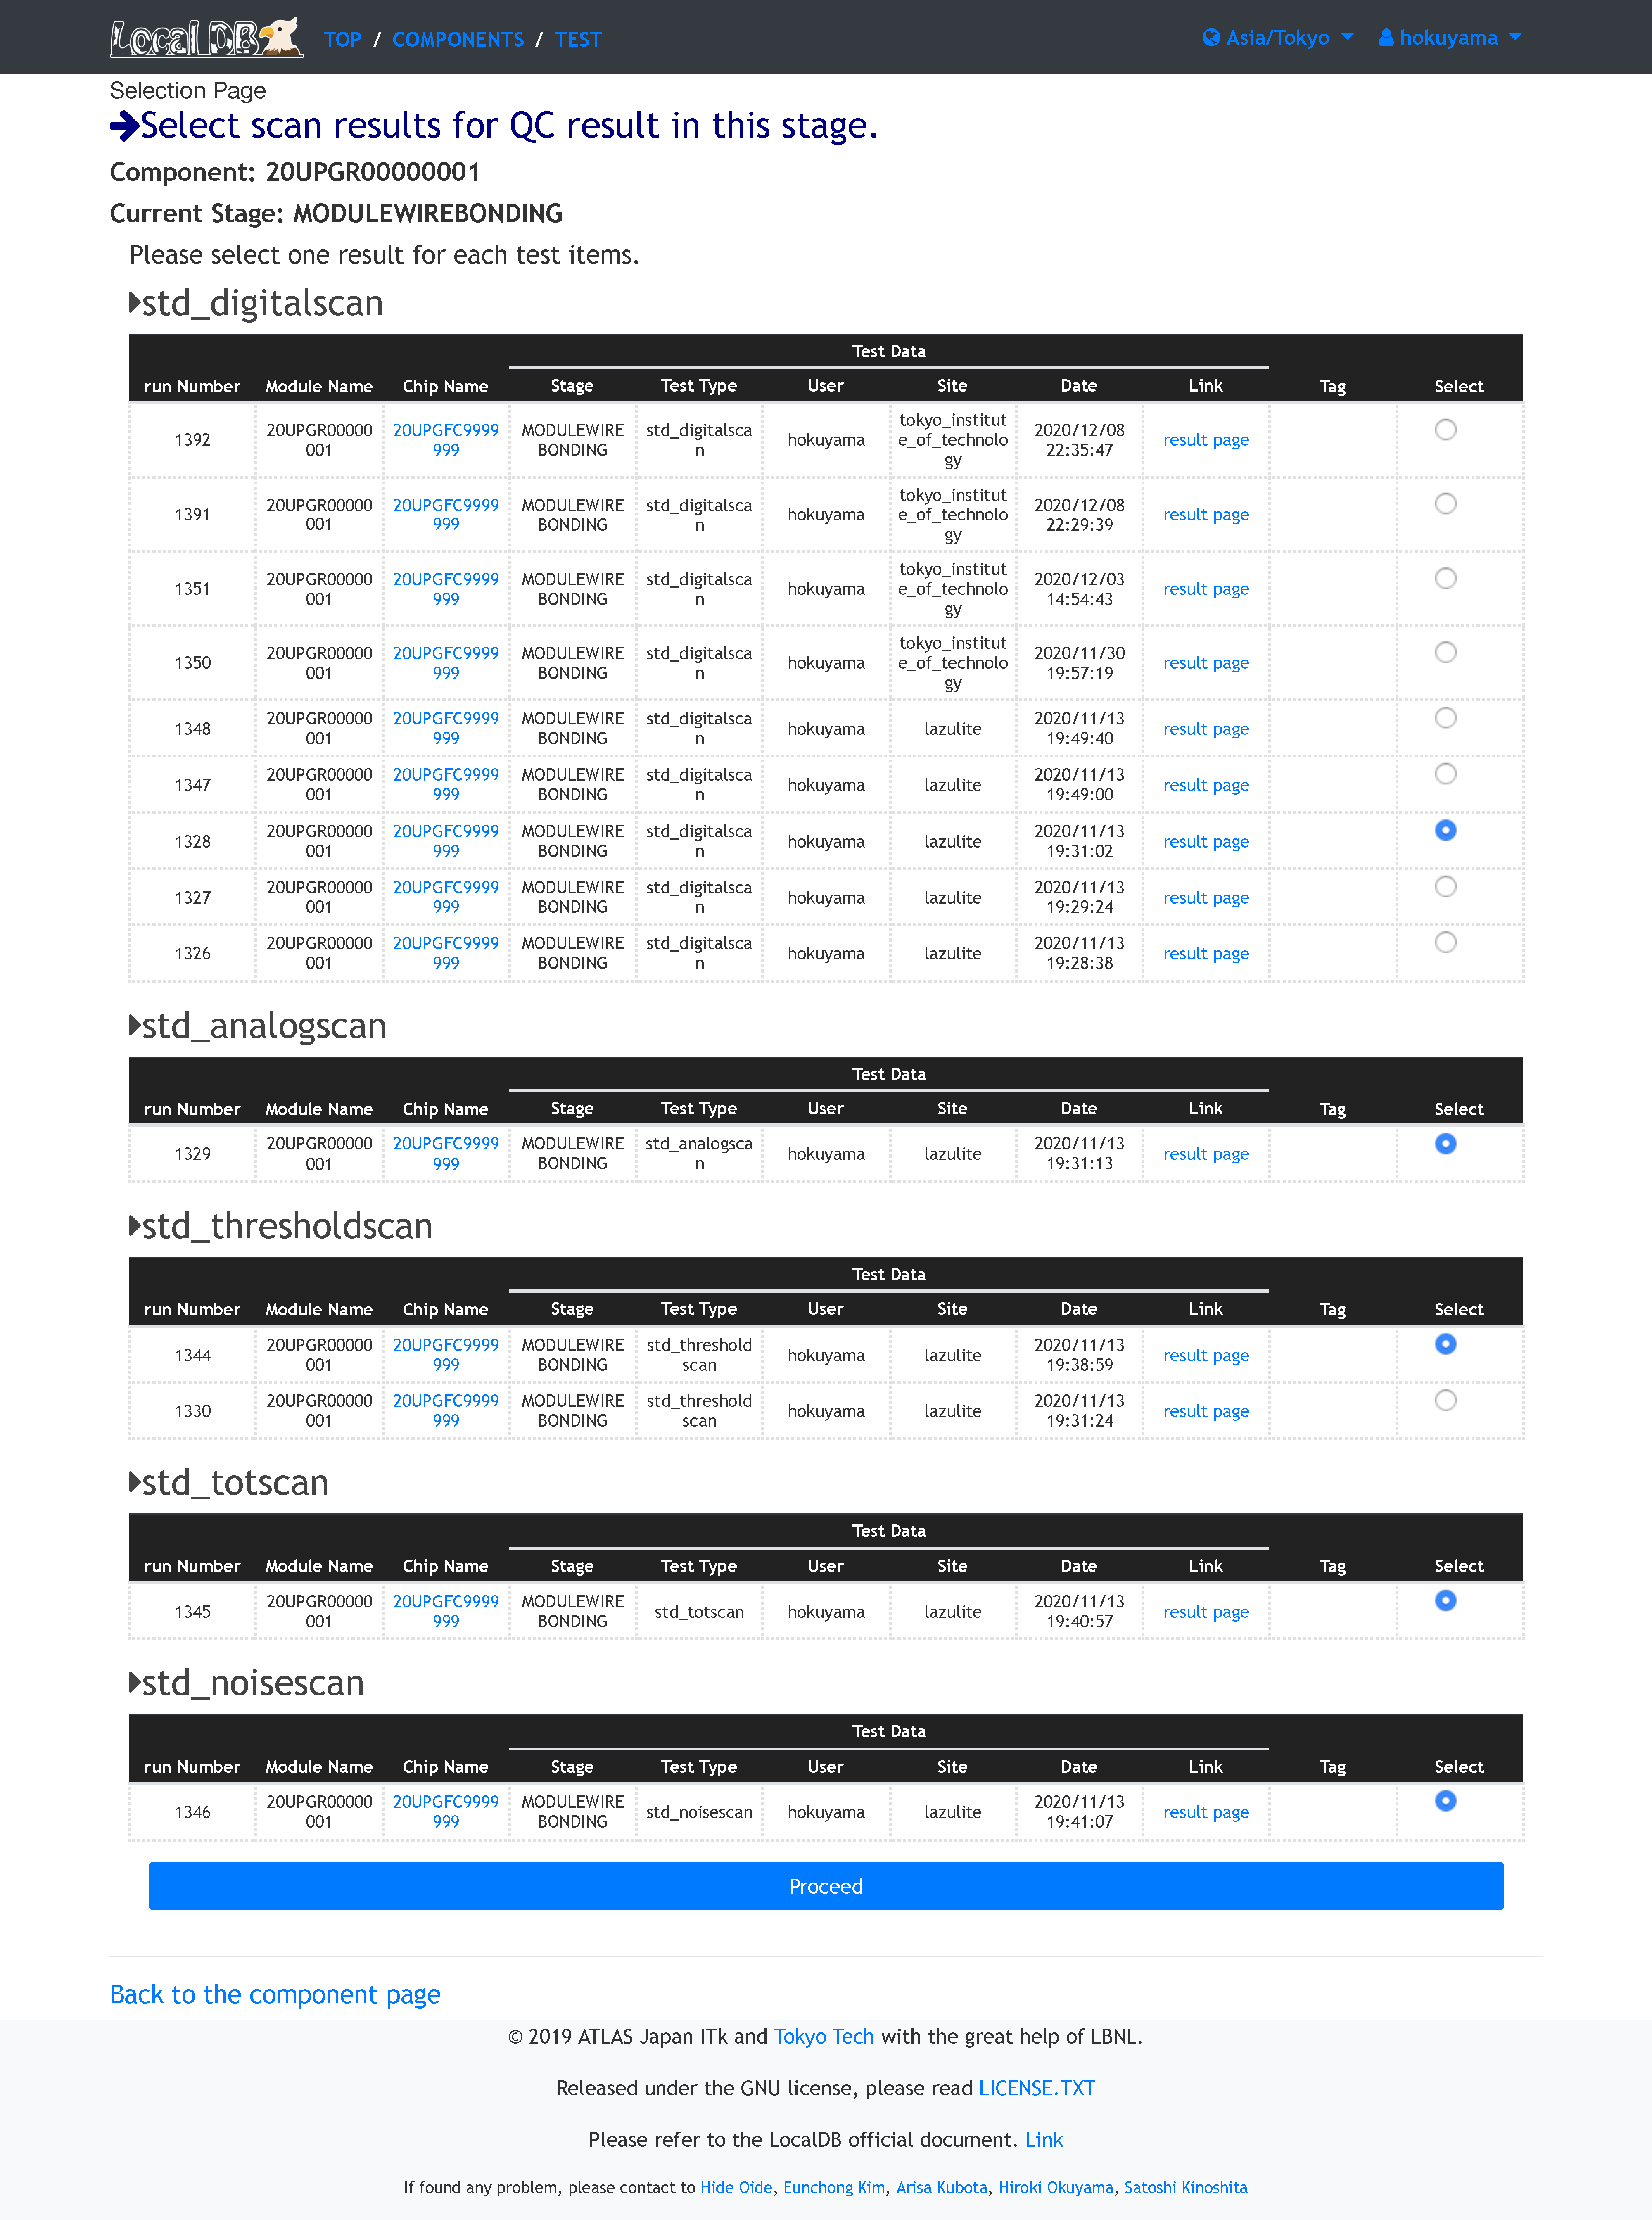
\includegraphics[width=10cm]{demo_select_scans}
  \caption[試験結果の選択]{試験結果の選択}
  \label{demo_select_scans}
  \end{center}
\end{figure}

不良評価基準は3章に述べた表\ref{pixel_analysis_criteria}の中から、基準が現時点で明確な以下の項目を選んだ。
\begin{itemize}
  \item Digital Dead 
  \item Digital Bad 
  \item Analog Dead 
  \item Analog Bad 
  \item Tuning Failed
  \item Tuning Bad for Threshold
  \item Tuning Bad for ToT
  \item High ENC
  \item Noisy
\end{itemize}

解析結果を表\ref{pixel_analysis_result}、図\ref{pixel_analysis_result_figure}に示す。
\begin{table}[tbp]
\begin{center}
\caption[ピクセル解析結果]{ピクセル解析結果}
\label{pixel_analysis_result}
  \begin{tabular}{|ll|} \hline
    1 & 2 \\ \hline
    result 1 & result 2 \\ \hline 
  \end{tabular}
\end{center}
\end{table}

\begin{figure}[bpt]\centering

\includegraphics[width=10cm]{figure}
\caption[ピクセル解析結果プロット]{ピクセル解析結果プロット}
\label{pixel_analysis_result_figure}
\end{figure}

%%%%%%%%%%%%%%%%%%%%%%%%%%%%%%%%%%%%%%%%%%%%%%%%%
%%%%%%%%%%%%%%%%%%%%%%%%%%%%%%%%%%%%%%%%%%%%%%%%%
\newpage
\subsubsection{試験結果アップロード}
選択した結果を中央データベースにアップロードし、各ファイルが正しくアップロードされていることを確認した。
各ファイルの存在を確認した結果を表\ref{scan_upload_pd}に示す。

